\documentclass[11pt,a4paper]{article}
\usepackage[T1]{fontenc}
\usepackage[utf8]{inputenc}
\usepackage{lmodern}
\usepackage{geometry}
\usepackage{graphicx}
\usepackage{booktabs}
\usepackage{amsmath}
\usepackage{siunitx}
\usepackage{float}
\usepackage{hyperref}
\usepackage[numbers,sort&compress]{natbib}
\usepackage{enumitem}
\geometry{margin=1in}
\hypersetup{colorlinks=true,linkcolor=blue,citecolor=blue,urlcolor=blue}
\setlist[itemize]{leftmargin=1.5em}
\title{VEHRON: a modular forward-time vehicle simulation framework for BEV energy, thermal, and subsystem studies}
\author{Subramanyam Natarajan}
\date{April 17, 2026}

\begin{document}
\maketitle

\begin{abstract}
VEHRON (VEHicle Research and Optimisation Network) is an open-source Python framework for forward-time road-vehicle simulation with an active focus on battery-electric passenger vehicles. The software is organized around a small orchestration core, a shared state bus, validated YAML configuration, and interchangeable subsystem modules for driver, longitudinal dynamics, drivetrain reduction, electric motor, inverter, regenerative braking, battery, HVAC, auxiliary loads, and low-order thermal trends. The current repository emphasizes engineering usability: reproducible case packaging, swappable battery and HVAC slots, fixed-step multi-rate execution, live run telemetry, and exported plots suitable for quick study review. This paper documents the present software architecture, the implemented model set, and representative outputs from highway and stop-start cycles. The manuscript is written as a software paper and preprint-style companion for eventual archival release and adaptation to Journal of Open Source Software submission requirements.
\end{abstract}

\section{Summary}
VEHRON is a component-based vehicle simulator designed for engineering studies such as energy consumption estimation, state-of-charge (SoC) trajectory prediction, thermal trend inspection, and comparison of operating cases across vehicle configurations. The project uses a forward-time simulation loop rather than a monolithic block diagram. A central software coordinator advances time and applies module outputs, while each module owns a bounded physical domain. In the current validated path, VEHRON assembles a battery-electric four-wheeler (BEV 4W) chain spanning speed tracking, longitudinal dynamics, drivetrain reduction, motor, inverter, regenerative braking, battery, HVAC, auxiliary loads, and low-order thermal management.

The repository has recently been extended from a mainly developer-oriented engineering MVP into a more usable run environment. The command-line entry point now prints a run ``spec sheet'' before simulation, streams live vehicle-level telemetry during execution at \SI{10}{\second} intervals, stores case packages under \texttt{output/cases/}, and generates post-run plots for motion, SoC with idle-state indication, and thermal channels. The full automated suite currently reports 25 passing tests in this workspace, including a runner integration test that checks the case package and plot outputs.

\section{Statement of Need}
Vehicle-simulation workflows often sit at an uncomfortable boundary. High-fidelity tools can be expensive, difficult to extend, or awkward to automate, while ad hoc spreadsheets and one-off scripts rarely scale into reusable research software. VEHRON is intended for users who need a transparent simulation stack that can be inspected, modified, and gradually upgraded without rewriting the whole loop each time a subsystem model changes. The current codebase is particularly aimed at:

\begin{itemize}
\item early-stage BEV sizing and trade studies,
\item subsystem sensitivity checks for battery, HVAC, and auxiliary loads,
\item repeatable comparison across route and environment cases,
\item integration of proprietary battery or HVAC models without committing the proprietary source into the repository.
\end{itemize}

This last point is one of VEHRON's differentiators. The repository includes in-repo reference models, but the battery and HVAC slots are explicit interfaces. A third-party pack model can be loaded at runtime from a local Python file if it inherits from the VEHRON base class, allowing proprietary electro-thermal logic to run inside an otherwise open vehicle-level simulation workflow.

\section{Software Architecture}
The present software architecture follows four rules. First, \texttt{SimEngine} owns orchestration and time stepping only; it does not carry subsystem physics internally. Second, \texttt{SimState} is the shared state bus between modules. Third, each module returns only the outputs it computes. Fourth, vehicle hardware and mission definitions are provided through validated YAML configuration rather than ad hoc runtime code.

At a high level, one run proceeds as follows:
\begin{enumerate}
\item vehicle YAML and testcase YAML are loaded and validated,
\item boundary-unit conversions are applied at the loader edge,
\item \texttt{SimEngine} instantiates the configured modules,
\item the engine advances the master clock and schedules modules according to their execution divisors,
\item module outputs are written back onto \texttt{SimState},
\item energy bookkeeping, logging, and termination checks are applied,
\item a flat time series and case package are emitted for post-processing.
\end{enumerate}

This separation keeps the core runtime small while allowing subsystems to evolve independently. It also makes the flat time-series export natural rather than an afterthought, which is useful for study logging, pack-team exports, and case packaging.

\subsection{Fixed-step multi-rate execution}
VEHRON uses a fixed-step master clock with per-module execution divisors. If the master timestep is $\Delta t$ and a module declares a divisor $d$, then its effective update interval is
\begin{equation}
\Delta t_{\mathrm{eff}} = d \, \Delta t.
\end{equation}
Fast domains such as the driver, longitudinal dynamics, motor, inverter, and regenerative braking run every master step in the active BEV chain, while slower domains such as battery electrical updates, HVAC, and thermal trends run less often. To avoid physically meaningless snapshots for slow modules, VEHRON calls \texttt{accumulate()} on every master step and \texttt{flush\_accumulator()} immediately before the scheduled update of the slower module. This lets slow modules use interval-averaged or interval-summed inputs instead of a single instantaneous value.

\subsection{Shared state contract}
The current shared state contains the motion variables, battery variables, motor variables, key temperatures, power channels, and cumulative energy channels needed by the active BEV path. Important state conventions include SI internal units, Kelvin for temperature, positive battery current for discharge, positive battery power for battery-side discharge, and positive regenerative power for energy recovered into the battery boundary.

\section{Implemented Models}
\subsection{Driver and longitudinal dynamics}
The active driver model is a PID-style speed tracker. With speed error
\begin{equation}
e(t) = v_{\mathrm{target}}(t) - v(t),
\end{equation}
the controller command is
\begin{equation}
u(t) = K_p e(t) + K_i \int e(t)\,dt + K_d \frac{de(t)}{dt},
\end{equation}
which is split into non-negative throttle and brake requests by clamping positive and negative command branches separately.

The longitudinal dynamics module then evaluates the net force
\begin{equation}
F_{\mathrm{net}} =
F_{\mathrm{trac}} - F_{\mathrm{brake}} - F_{\mathrm{aero}} - F_{\mathrm{roll}} - F_{\mathrm{grade}},
\end{equation}
with acceleration
\begin{equation}
a = \frac{F_{\mathrm{net}}}{m}.
\end{equation}
The current implementation represents aerodynamic drag as
\begin{equation}
F_{\mathrm{aero}} = \frac{1}{2}\rho C_d A v_{\mathrm{rel}}^2,
\end{equation}
and rolling plus grade loads as low-order functions of mass, road grade, and speed. This is a simple but effective road-load closure for whole-vehicle energy studies.

\subsection{Motor, inverter, and regenerative braking}
The default analytical motor model clamps torque and mechanical power to the configured peak limits and computes a low-order efficiency estimate from load fraction and speed fraction. For motoring operation, electrical drive demand is estimated from mechanical power and the motor efficiency, then passed through an inverter stage with configurable efficiency. Regenerative braking is modeled as a blended brake controller that limits recovered power by both the requested braking level and the instantaneous kinetic power available at the wheel boundary.

\subsection{Battery models}
VEHRON currently carries two in-repo battery models. The baseline \texttt{Rint} model provides lightweight SoC and terminal-voltage behavior suitable for quick energy studies. The higher-fidelity two-RC ECM model introduces an open-circuit voltage estimate and two polarization branches, following the widely used equivalent-circuit modeling family for lithium-ion batteries \citep{hu2012ecm,su2019ecm}. Conceptually,
\begin{equation}
V_{\mathrm{term}} = V_{\mathrm{ocv}} - I R_0 - V_{\mathrm{rc1}} - V_{\mathrm{rc2}}.
\end{equation}
Each RC branch relaxes toward its current-dependent equilibrium with its own time constant,
\begin{equation}
\tau_i = R_i C_i.
\end{equation}
The current implementation uses a stable exponential update for these branch states. Both in-repo battery models expose SoC, battery current, terminal voltage, and net battery power. Both also accept optional external charging power as an input channel, though a full automatic stop-charge-resume mission controller has not yet been implemented in the runtime.

The battery slot is a formal interface rather than a hard-coded in-repo dependency. This means a proprietary pack model can be loaded from a local Python file at runtime as long as it inherits from the VEHRON battery base class. The same approach exists for HVAC.

\subsection{Cabin HVAC and thermal trends}
The cabin HVAC model is a low-order lumped thermal model aligned with the standard vehicle-cabin thermal-model family used for energy studies \citep{marcos2014cabin,torregrosa2015cabin,noreen2019thermal,cabreview2024}. The present formulation decomposes the thermal load into envelope exchange, solar gain, ventilation or fresh-air load, occupant sensible load, and HVAC-delivered heat:
\begin{equation}
Q_{\mathrm{net}} =
Q_{\mathrm{envelope}} +
Q_{\mathrm{solar}} +
Q_{\mathrm{ventilation}} +
Q_{\mathrm{occupants}} +
Q_{\mathrm{hvac}}.
\end{equation}
Cabin temperature then evolves according to
\begin{equation}
\frac{dT_{\mathrm{cabin}}}{dt} = \frac{Q_{\mathrm{net}}}{C_{\mathrm{total}}},
\end{equation}
and HVAC electrical power is estimated from the thermal load and the relevant coefficient of performance. Battery, motor, and coolant temperatures are presently represented by low-order trend models rather than high-resolution thermal networks. This is a deliberate trade-off to keep the whole-vehicle loop fast while still exposing thermal behavior at the vehicle level.

\section{Representative Workflows and Outputs}
The command-line workflow now exposes more of the run to the user than the earlier CLI summary. Before execution, VEHRON prints a test specification sheet containing the vehicle, testcase, route mode, environment, battery configuration, and simulation settings. During execution, it prints vehicle-level progress at \SI{10}{\second} intervals, including distance traveled, speed, acceleration, SoC, and available temperatures such as ambient, motor, battery, coolant, and cabin temperatures. After execution, the runtime writes a case package containing:

\begin{itemize}
\item \texttt{summary.json},
\item \texttt{timeseries.csv},
\item copied input YAML files,
\item resolved YAML snapshots,
\item generated plots,
\item a brief case README.
\end{itemize}

\begin{figure}[H]
\centering
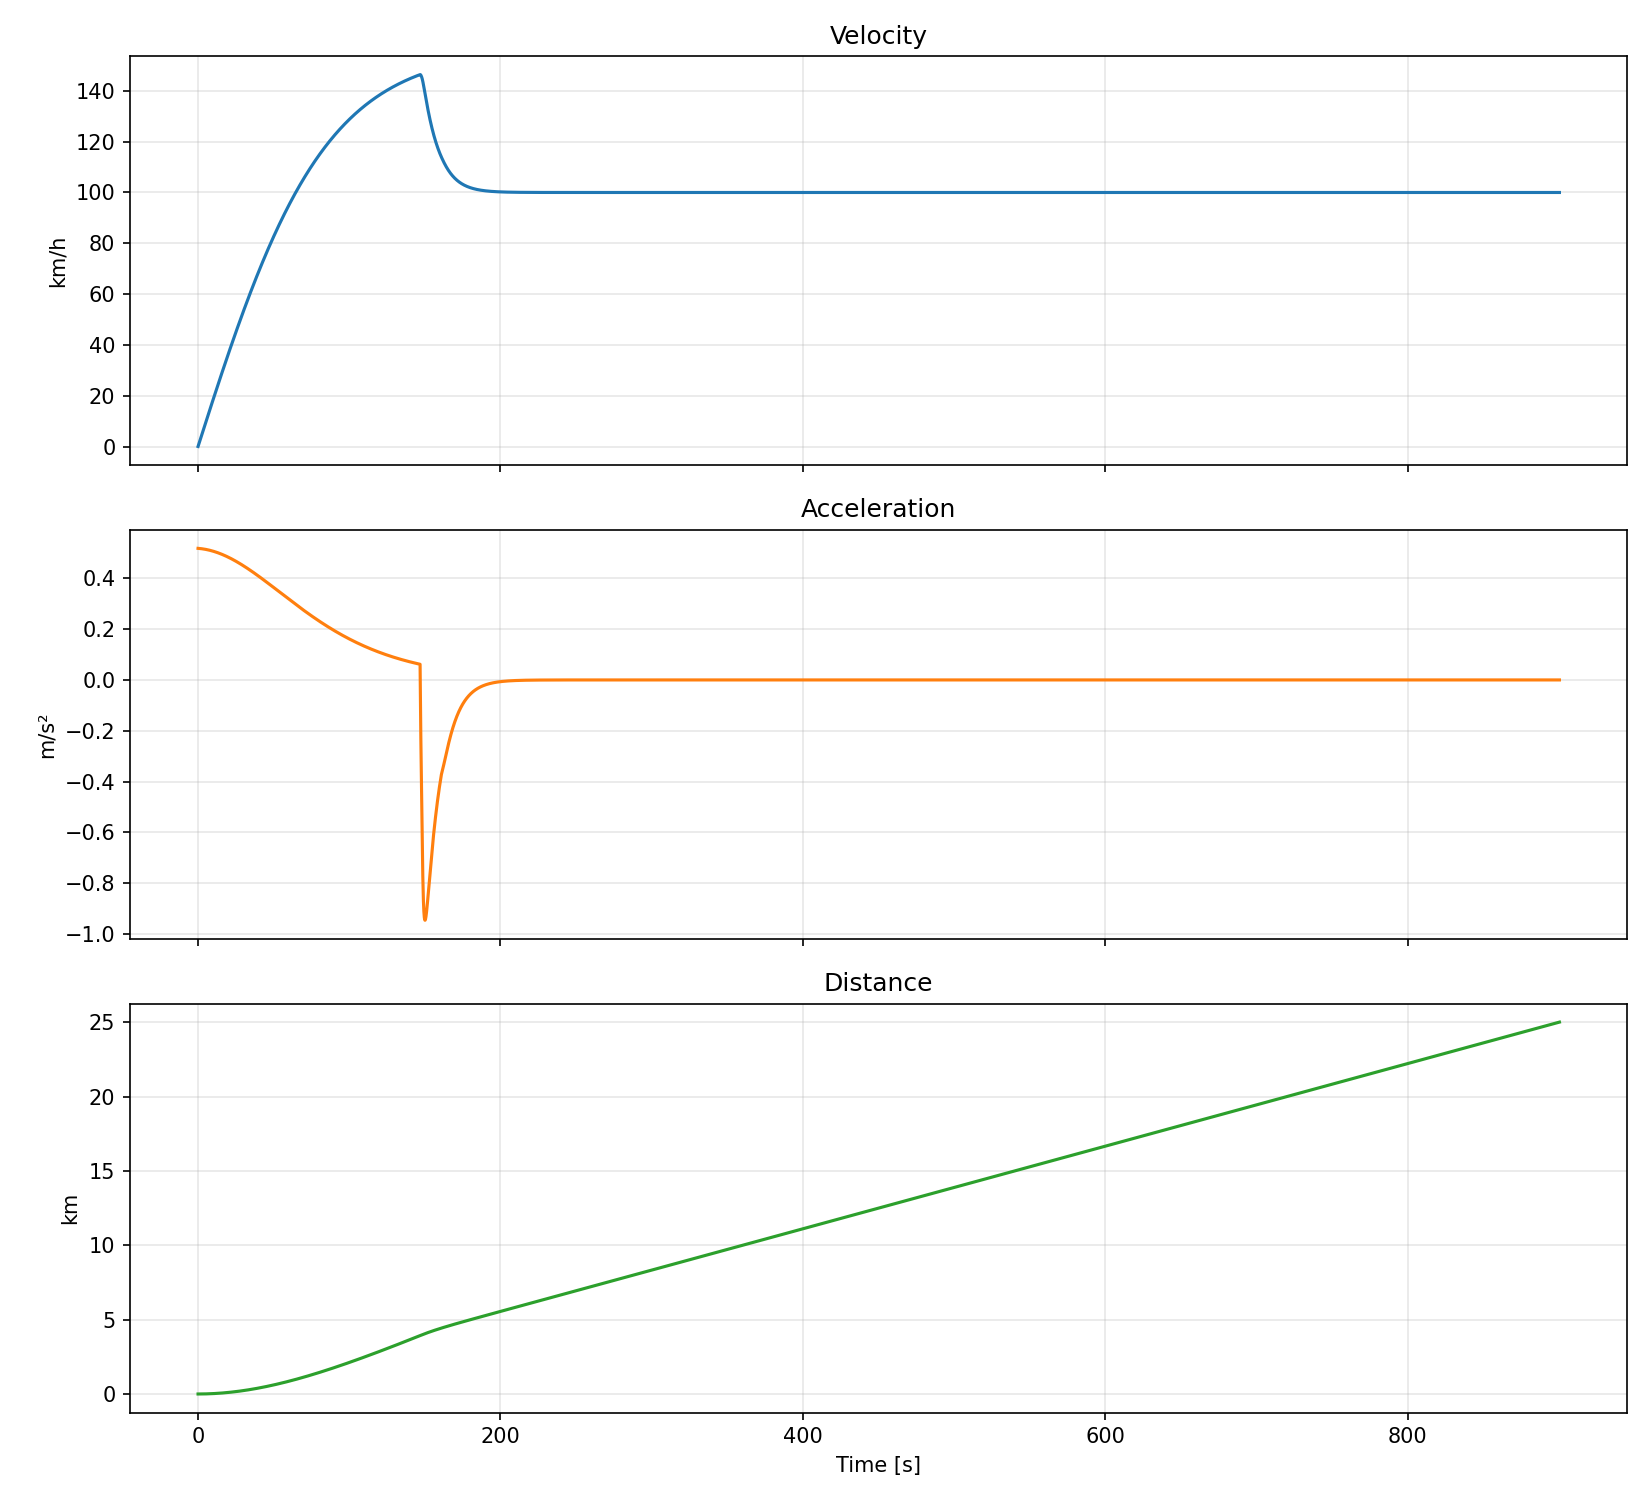
\includegraphics[width=0.92\linewidth]{figures/highway_motion.png}
\caption{Motion channels from the default flat-highway BEV case. The case package includes velocity, acceleration, and distance traces together in one plot.}
\label{fig:highway_motion}
\end{figure}

\begin{figure}[H]
\centering
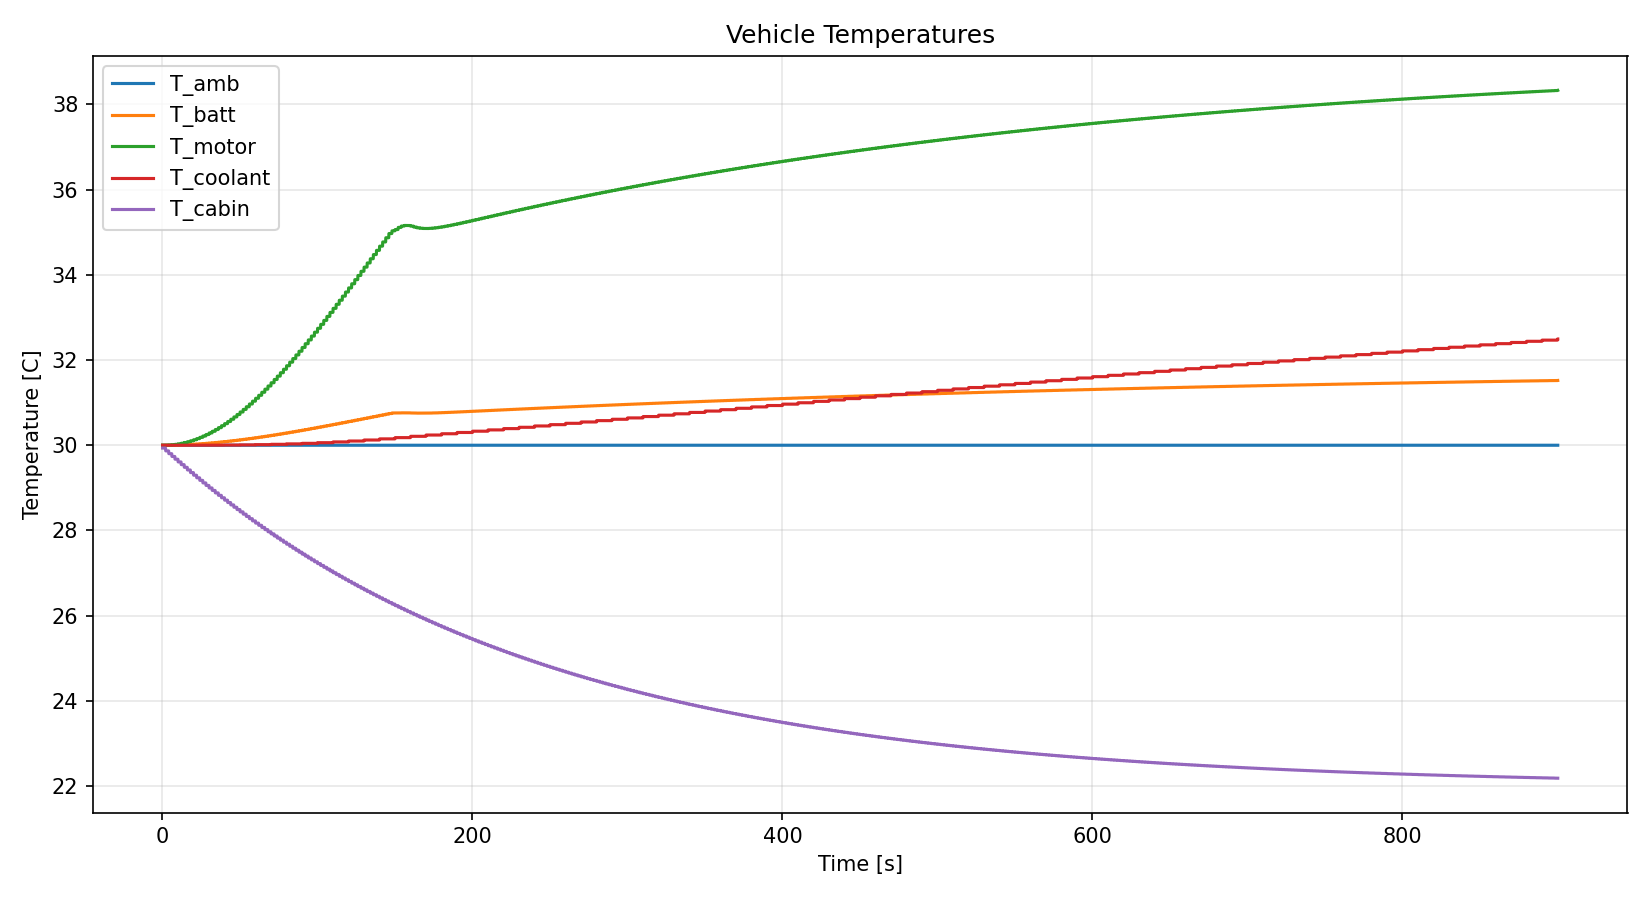
\includegraphics[width=0.92\linewidth]{figures/highway_temperatures.png}
\caption{Vehicle temperature channels from the same highway case. The current built-in plots expose ambient, battery, motor, coolant, and cabin temperature trajectories.}
\label{fig:highway_temp}
\end{figure}

\begin{figure}[H]
\centering
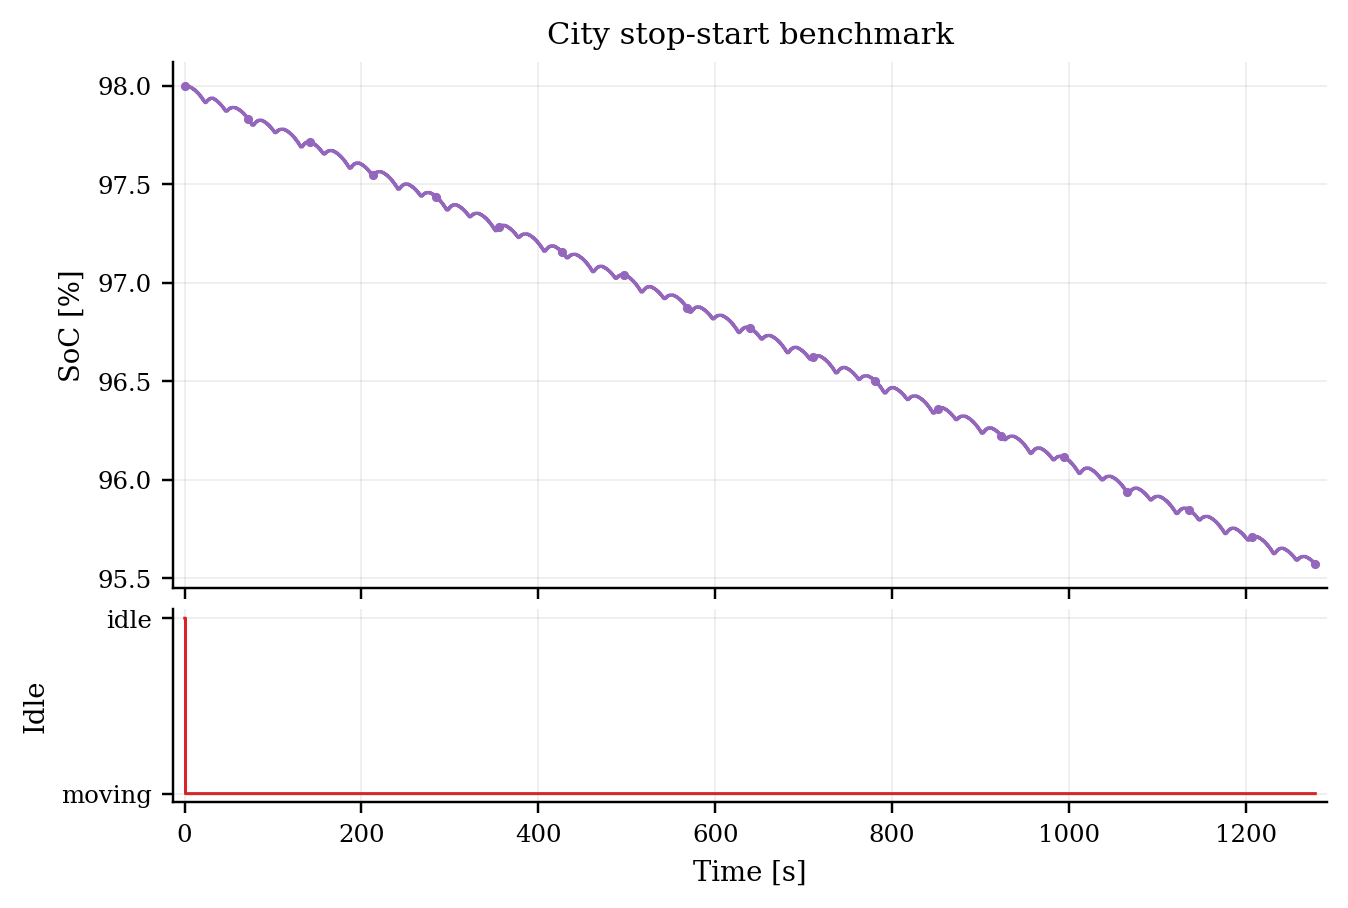
\includegraphics[width=0.92\linewidth]{figures/city_soc_idle.png}
\caption{SoC and idle-state plot for the WLTP-like stop-start city cycle. This case shows repeated regenerative events and a smaller net SoC drop than the flat-highway case.}
\label{fig:city_soc}
\end{figure}

Two current reference runs illustrate the present behavior. The flat-highway \SI{100}{\kilo\meter\per\hour} BEV sedan case covers \SI{25.0}{\kilo\meter} in about \SI{900}{\second}, with a SoC drop from 0.98 to about 0.887 and a net energy use of roughly \SI{5.10}{\kilo\watt\hour}. The WLTP-like stop-start city case covers just over \SI{8.0}{\kilo\meter} with a SoC drop from 0.98 to about 0.956 and accumulates substantially more regenerative recovery, which is visible in the city-cycle SoC behavior and the regenerated-energy total.

\begin{table}[H]
\centering
\caption{Representative current case summaries generated by VEHRON case packages.}
\label{tab:cases}
\resizebox{\linewidth}{!}{%
\begin{tabular}{lrrrrr}
\toprule
Case & Distance (km) & Final SoC & Energy (Wh) & Regen (Wh) & Final $T_{\mathrm{motor}}$ (C) \\
\midrule
Flat highway 100 km/h & 25.001 & 0.8872 & 5103.6 & 33.4 & 38.33 \\
City WLTP-like stop-start & 8.001 & 0.9557 & 1337.1 & 691.8 & 31.27 \\
\bottomrule
\end{tabular}
\par}
\end{table}

\section{Current Limitations and Next Steps}
VEHRON is still an engineering MVP. The in-repo battery models are low-order pack models rather than full electrochemical solvers. Thermal behavior is tracked at pack, motor, coolant, and cabin trend level rather than through resolved cell-core or condenser and radiator models. The active route inputs are parametric cases and CSV drive cycles; a GPX-derived mission path discussed during this development session would be a natural next addition, ideally followed by an inverse-replay mode that derives wheel demand directly from measured motion rather than from a controller tracking a reference.

The runtime now supports case packaging, live telemetry, plots, and export hooks, but several roadmap items remain important:
\begin{itemize}
\item a mission controller for automatic stop-charge-resume behavior,
\item richer standardized thermal telemetry for pluggable devices,
\item GPX route ingestion and trace replay,
\item stronger energy-balance and end-to-end integration checks beyond the current basic integration tests,
\item final alignment with JOSS submission packaging, which uses \texttt{paper.md} rather than LaTeX as the formal submission format.
\end{itemize}

\section{Availability}
VEHRON is distributed as Python source under the AGPL-3.0-only license in this repository. The present workspace includes automated tests, example archetypes and testcases, case-package generation, and a manuscript folder with generated figures. The code is intended to be archived with a DOI-bearing software release for eventual Zenodo deposition and adapted into the exact Journal of Open Source Software submission format when the project is ready for formal review.

\section{Acknowledgements}
The project reflects sustained personal engineering effort toward an open, modular vehicle-simulation stack that can host both in-repo and externally supplied subsystem models. The recent CLI and reporting improvements documented here were developed directly against the current repository and validated with the local test suite.

\bibliographystyle{plainnat}
\bibliography{vehron_refs}

\end{document}
